\graphicspath{{Figures/}}

\title{\fontsize{33}{45}{\huge Pattern Classification\newline \vspace{8pt} \Large \vspace{-1.1cm}}}

\vspace{0.5cm}
\author{\vspace{0.4cm}\\\large{\bf Kundan Kumar\\\url{https://github.com/erkundanec/PatternClassification}}
%Associate Professor\\Department of ECE}
}
% - Give the names in the same order as the appear in the paper.
% - Use the \inst{?} command only if the authors have different
%   affiliation.
%\vspace{1cm}
\institute[Indian Institute of Technology Kharagpur] % (optional, but mostly needed)
{
\vspace{1.8cm}
%\includegraphics[height=.17\textheight]{SOAlogo.png}\\
% Faculty of Engineering (ITER)\\ S`O'A Deemed to be University, Bhubaneswar, India-751030\\


 \copyright\  2020 Kundan Kumar, All Rights Reserved\\
  \vspace{-1.1cm}}
% - Use the \inst command only if there are several affiliations.
% - Keep it simple, no one is interested in your street address.
\date{}
% To remove page number from a perticular slide
{
\setbeamertemplate{logo}{}
\makeatletter
\setbeamertemplate{footline}{
        \leavevmode%
  
  % First line.
  \hbox{%
  \begin{beamercolorbox}[wd=.2\paperwidth,ht=\beamer@decolines@lineup,dp=0pt]{}%
  \end{beamercolorbox}%
  \begin{beamercolorbox}[wd=.8\paperwidth,ht=\beamer@decolines@lineup,dp=0pt]{lineup}%
  \end{beamercolorbox}%
  } %
  % Second line.
  \hbox{%
  \begin{beamercolorbox}[wd=\paperwidth,ht=\beamer@decolines@linemid,dp=0pt]{linemid}%
  \end{beamercolorbox}%
  } %
  % Third line.
  \hbox{%
  \begin{beamercolorbox}[wd=.1\paperwidth,ht=\beamer@decolines@linebottom,dp=0pt]{}%
  \end{beamercolorbox}%
  \begin{beamercolorbox}[wd=.9\paperwidth,ht=\beamer@decolines@linebottom,dp=0pt]{linebottom}%
  \end{beamercolorbox}%
  }%
        }
\makeatother
\begin{frame}
\titlepage
\end{frame}
}

\section{Introduction}
\subsection{}
\begin{frame}{}
\begin{variableblock}{\centering \Large \textbf{\vspace{4pt}\newline Unsupervised Learning: Clustering\vspace{4pt}}}{bg=slidecolor,fg=white}{bg=slidecolor,fg=white}
\end{variableblock}
\end{frame}

\begin{frame}{Introduction}
\begin{itemize}
\item In previous lectures, we have seen that how samples are classified if a training set is available along with class labels to design a classifier.
\item In many situations, class labels are not known for the training samples.
\item The area of pattern classification which {\color{mycolor1}cluster / group the data samples} based on some {\color{mycolor1}similarity} is known as {\color{mycolor2}clustering}.
\item Clustering refers to the process of grouping samples so that the samples are similar within each group. The groups are called \textit{\color{mycolor2}clusters}.
\end{itemize}
\end{frame}

\section{Hierarchical Clustering}
\subsection{}
\begin{frame}{Hierarchical Clustering}
\begin{itemize}
\item Hierarchical clustering refers to a clustering process that organizes the data into large groups, which contain smaller groups, and so on.
\item Hierarchical clustering approach can be categorize as
\begin{itemize}
\item Bottom-Up approach (called \textit{\color{slidecolor}Agglomerative} clustering)
\item Top-Down approach (called \textit{\color{slidecolor}Divisive} clustering)
\end{itemize}
\item A hierarchical clustering may be drawn as a \textit{\color{slidecolor}tree} or \textit{\color{slidecolor}dendrogram}.
\end{itemize}
\end{frame}

\begin{frame}{Agglomerative Clustering}
\begin{itemize}
\setlength{\itemsep}{12pt}
\item Consider ${\rm x}_1,{\rm x}_2,\ldots,{\rm x}_n$ are $n$ $d$-dimensional feature vectors.
\item Algorithm:
\begin{itemize}
\item[1:] Begin with $n$ clusters, each consisting of one sample.
\item[2:] Repeat step 3 a total of $n-1$ times
\item[3:] Find the most similar clusters $C_i$ and $C_j$ and merge $C_i$ and $C_j$ into one cluster. If there is a tie, merge the first pair found.
\end{itemize}
\end{itemize}
\end{frame}

\begin{frame}{Agglomerative Clustering}
\begin{itemize}
\item Agglomerative clustering can be performed using these approach:
\begin{itemize}
\item Single-linkage algorithm
\begin{equation}
D_{SL}(C_i,C_j)=\min_{a\in C_i,b\in C_j}{d(a,b)} \nonumber
\end{equation}
\item Complete-linkage algorithm
\begin{equation}
D_{SL}(C_i,C_j)=\max_{a\in C_i,b\in C_j}{d(a,b)} \nonumber
\end{equation}
\item Average-linkage algorithm
\begin{equation}
D_{SL}(C_i,C_j)=\mathop {\rm avg}\limits_{a\in C_i,b\in C_j}{d(a,b)} \nonumber
\end{equation}
\end{itemize}
\end{itemize}
\end{frame}



\begin{frame}{Example: Single-linkage algorithm}
\textit{\color{slidecolor}Question 01:} Perform a hierarchical clustering of five samples using the single-linkage algorithm and two features $x$ and $y$.
\begin{figure}
\includegraphics[scale=0.13]{cluster08.JPG}
\end{figure}
\begin{itemize}
\item Combine 1 and 2 in single cluster
\begin{equation}
\{1,2\},\{3\},\{4\},\{5\}\nonumber
\end{equation}
\end{itemize}
\end{frame}

\begin{frame}{Example: Single-linkage algorithm}
\begin{figure}
\includegraphics[scale=0.1]{cluster09.JPG}
\end{figure}
\begin{itemize}
\item Minimum value is 8.0 so merge cluster $\{4\}$ and $\{5\}$.
\begin{equation}
\{1,2\},\{3\},\{4,5\}\nonumber
\end{equation}
\end{itemize}
\end{frame}

\begin{frame}{Example: Single-linkage algorithm}
\begin{columns}
\begin{column}{5.5cm}
\begin{figure}
\includegraphics[scale=0.1]{cluster10.JPG}
\end{figure}
\begin{itemize}
\item Minimum value is 8.1 so merge cluster $\{1,2\}$ and $\{3\}$.
\begin{equation}
\{1,2,3\},\{4,5\}\nonumber
\end{equation}
\item In next step will merge the two remaining clusters at a distance of 9.8.
\end{itemize}
\end{column}
\begin{column}{5.5cm}
\begin{figure}
\includegraphics[scale=0.1]{cluster14.JPG}
\caption{Dendrogram of Hierarchical clustering using single-linkage algorithm}
\end{figure}
\end{column}
\end{columns}
\end{frame}

\begin{frame}{Example: Complete-linkage algorithm}
\textit{\color{slidecolor}Question 02:} Perform a hierarchical clustering of five samples using the complete-linkage algorithm and two features $x$ and $y$.
\begin{figure}
\includegraphics[scale=0.13]{cluster08.JPG}
\end{figure}
\begin{itemize}
\item Combine 1 and 2 in single cluster
\begin{equation}
\{1,2\},\{3\},\{4\},\{5\}\nonumber
\end{equation}
\end{itemize}
\end{frame}

\begin{frame}{Example: Complete-linkage algorithm}
\begin{figure}
\includegraphics[scale=0.33]{cluster11.JPG}
\end{figure}
\begin{itemize}
\item Minimum value is 8.0 so merge cluster $\{4\}$ and $\{5\}$.
\begin{equation}
\{1,2\},\{3\},\{4,5\}\nonumber
\end{equation}
\end{itemize}
\end{frame}

\begin{frame}{Example: Complete-linkage algorithm}
\begin{columns}
\begin{column}{5cm}
\begin{figure}
\includegraphics[scale=0.1]{cluster12.JPG}
\end{figure}
\begin{itemize}
\item Minimum value is 9.8 so merge cluster $\{4,5\}$ and $\{3\}$.
\begin{equation}
\{1,2\},\{3,4,5\}\nonumber
\end{equation}
\item In next step will merge the two remaining clusters.
\end{itemize}
\end{column}
\begin{column}{5.5cm}
\begin{figure}
\includegraphics[scale=0.1]{cluster13.JPG}
\caption{Dendrogram of Hierarchical clustering using complete-linkage algorithm}
\end{figure}
\end{column}
\end{columns}
\end{frame}

\begin{frame}{Example: Average-linkage algorithm}
\textit{\color{slidecolor}Question 03:} Perform a hierarchical clustering of five samples using the average-linkage algorithm and two features $x$ and $y$.
\begin{figure}
\includegraphics[scale=0.13]{cluster08.JPG}
\end{figure}
\begin{itemize}
\item Combine 1 and 2 in single cluster
\begin{equation}
\{1,2\},\{3\},\{4\},\{5\}\nonumber
\end{equation}
\end{itemize}
\end{frame}

\begin{frame}{Example: Average-linkage algorithm}
\begin{figure}
\includegraphics[scale=0.13]{cluster30.JPG}
\end{figure}
\begin{itemize}
\item Minimum value is 8.0 so merge cluster $\{4\}$ and $\{5\}$.
\begin{equation}
\{1,2\},\{3\},\{4,5\}\nonumber
\end{equation}
\end{itemize}
\end{frame}

\begin{frame}{Example: Average-linkage algorithm}
\begin{columns}
\begin{column}{5cm}
\begin{figure}
\includegraphics[scale=0.12]{cluster31.JPG}
\end{figure}
\begin{itemize}
\item Minimum value is 9.8 so merge cluster $\{4,5\}$ and $\{3\}$.
\begin{equation}
\{1,2\},\{3,4,5\}\nonumber
\end{equation}
\item In next step will merge the two remaining clusters.
\end{itemize}
\end{column}
\begin{column}{5.5cm}
\begin{figure}
\includegraphics[scale=0.1]{cluster32.JPG}
\caption{Dendrogram of Hierarchical clustering using average-linkage algorithm}
\end{figure}
\end{column}
\end{columns}
\end{frame}


\begin{frame}{Ward's Algorithm}
\begin{itemize}
\item The hierarchical clustering based on variance.
\item also called minimum-variance method
\item Consider $C_j$ class has $n$ no. of feature vectors ${\rm x}_1,{\rm x}_2,\ldots,{\rm x}_n$
\item Error within $j^{th}$ cluster
\begin{equation}
{E_j} = \sum\limits_{i = 1}^n {{{\left\| {{{\rm x}_i} - \mu } \right\|}^2} = m{\sigma ^2}} \nonumber
\end{equation}
we need to minimize the variance
\item Total error
\begin{equation}
E=\sum\limits_{i = 1}^c E_j \nonumber
\end{equation}
\item Computationally expensive because need to check all combination of samples.
\end{itemize}
\end{frame}

\begin{frame}{Example: Ward's algorithm}
\vspace{-0.5cm}
\begin{columns}
\begin{column}{3cm}
\begin{figure}
\includegraphics[scale=0.15]{cluster16.JPG}
\end{figure}
\end{column}
\begin{column}{6.5cm}
\begin{figure}
\includegraphics[scale=0.13]{cluster15.JPG}
\end{figure}
\end{column}
\end{columns}
\vspace{12pt}
\begin{itemize}
\item Minimum Squared Error is 8.0 so form the cluster $\{1,2\},\{3\},\{4\},\{5\}$
\end{itemize}
\end{frame}

\begin{frame}{Example: Ward's algorithm}
\begin{figure}
\includegraphics[scale=.15]{cluster17.JPG}
\end{figure}
\begin{itemize}
\item Minimum Squared Error is 40.0 so form the cluster $\{1,2\},\{3\},\{4,5\}$
\end{itemize}
\end{frame}

\begin{frame}{Example: Ward's algorithm}
\begin{columns}
\begin{column}{5cm}
\begin{figure}
\includegraphics[scale=0.1]{cluster20.JPG}
\end{figure}
\begin{itemize}
\item Minimum value is 94.0 so form the cluster $\{1,2\},\{3,4,5\}$
\item In next step will merge the two remaining clusters.
\end{itemize}
\end{column}
\begin{column}{5.5cm}
\begin{figure}
\includegraphics[scale=0.1]{cluster21.JPG}
\caption{Dendrogram of Ward's algorithm}
\end{figure}
\end{column}
\end{columns}
\end{frame}


\begin{frame}{Batchelor and Wilkins' Algorithm}
\begin{itemize}
\item Heuristic procedure for clustering also called \textit{\color{slidecolor}maximum distance algorithm}
\begin{figure}
\includegraphics[scale=0.17]{cluster01.png}
\end{figure}
\end{itemize}
\end{frame}

\begin{frame}{Batchelor and Wilkins' Algorithm}
\begin{scriptsize}
\begin{itemize}
\item[Step 1:] Arbitrarily, let ${\rm x_1}$ be the first cluster center, designated by ${\rm z}_1$.
\item[Step 2:]Determine the pattern sample farthest from ${\rm x}_1$, which is ${\rm x}_6$. Call it cluster center ${\rm z}_6$.
\item[Step 3:] Compute the distance from each remaining pattern sample to ${\rm z}_1$ and ${\rm z}_2$
\item[Step 4:] Save the minimum distance for each pair of these computations.
\item[Step 5:] Select the maximum of these minimum distances.
\item[Step 6:] If the distance is appreciably greater than a fraction of the distance $d({\rm z}_1,{\rm z}_2)$, call the corresponding sample cluster center ${\rm z}_3$. Otherwise, the algorithm is terminated.

\item[Step 7:] If this distance from each of the three established cluster centers to the remaining samples and save the minimum of every group of three distances. Again select the maximum of these minimum distances. If this distance is an appreciable fraction of the ``typical'' previous maximum distances, the corresponding sample becomes cluster center ${\rm z}_4$. Otherwise, the algorithm is terminated.
\item[Step 8:] Repeat until the new maximum distance at a particular step fails to satisfy the condition for the creation of a new cluster center.
\item[Step 9:] Assign each sample to its nearest cluster center.
\end{itemize}
\end{scriptsize}
\end{frame}

\begin{frame}{Batchelor and Wilkins' Algorithm}
\begin{figure}
\includegraphics[scale=0.105]{cluster23.JPG}
\end{figure}
\end{frame}

\begin{frame}{Batchelor and Wilkins' Algorithm}
\begin{figure}
\begin{tikzpicture}[overlay,remember picture]
\draw[help lines,white] (-5,-3) grid (5,3);
\node at(-5,2.4){\pgftext{$A\rightarrow (1,1)$}};
\node at(-5,1.9){\pgftext{$B\rightarrow (1,2)$}};
\node at(-5,1.4){\pgftext{$C\rightarrow (3,2)$}};
\node at(-5,0.9){\pgftext{$D\rightarrow (3,3)$}};
\node at(-5,0.4){\pgftext{$E\rightarrow (6,6)$}};
\node at(-5,-0.1){\pgftext{$F\rightarrow (6,7)$}};
\node at(-5,-0.6){\pgftext{$G\rightarrow (7,6)$}};
\node at(-5,-1.1){\pgftext{$H\rightarrow (7,6)$}};
\node at(-5,-1.6){\pgftext{$I\rightarrow (7,1)$}};
\node at(-5,-2.1){\pgftext{$J\rightarrow (8,2)$}};
\node at(-5,-2.6){\pgftext{$K\rightarrow (9,1)$}};
\node at(1,0){\pgftext{\begin{footnotesize}
\begin{tabular}{p{0.4cm}|p{0.3cm}|p{0.3cm}|p{0.3cm}|p{0.3cm}|p{0.3cm}|p{0.3cm}|p{0.3cm}|p{0.4cm}|p{0.3cm}|p{0.3cm}|p{0.4cm}|}
&A&B&C&D&E&F&G&H&I&J&K\\\hline
A&0.0&1.0&2.2&2.8&7.0&7.8&7.8&8.48&6.0&7.0&8.0\\\hline
B&1.0&0.0&2.0&2.2&6.4&7.0&7.0&7.8&6.0&7.0&8.06\\\hline
C&&&&&&&&&&&\\\hline
D&&&&&&&&&&&\\\hline
E&&&&&&&&&&&\\\hline
F&&&&&&&&&&&\\\hline
G&&&&&&&&&&&\\\hline
H&&&&&&&&&&&\\\hline
I&&&&&&&&&&&\\\hline
J&&&&&&&&&&&\\\hline
K&&&&&&&&&&&\\\hline
\end{tabular}
\end{footnotesize}}};
\end{tikzpicture}
\end{figure}
\end{frame}

\begin{frame}{Batchelor and Wilkins' Algorithm}
\begin{figure}
\includegraphics[scale=0.105]{cluster25.JPG}
\end{figure}
\end{frame}

\begin{frame}{Batchelor and Wilkins' Algorithm}
\begin{figure}
\includegraphics[scale=0.085]{cluster24.JPG}
\end{figure}
Final clusters are $\{A,B,C,D\},\{E,F,G,H\},\{I,J,K\}$
\end{frame}

\section{Graph Based Clustering}
\subsection{}
\begin{frame}{Graph Based Clustering}
\begin{itemize}
\item Graph can be represented as
\begin{equation}
G = \left\langle {V,E} \right\rangle \nonumber
\end{equation}
where $V$ is set of nodes or vertices and $E$ is set of Edges.
\item There are many ways to represent a graph and one of them is similarity matrix
\item For $n$ number of nodes, similarity matix will be of size $n\times n$.
\item The elements of similarity matrix will be either 0 or 1.
\item $S(i,j)=1$, if $V_i$ and $V_j$ are connected in some sense. 
\end{itemize}
\end{frame}


\begin{frame}{Similarity Matrix based clustering}
\begin{figure}
\includegraphics[scale=0.105]{cluster23.JPG}
\end{figure}
\end{frame}

\begin{frame}{Similarity Matrix based clustering}
\begin{figure}
\includegraphics[scale=0.115]{cluster27.JPG}
\end{figure}
\end{frame}

\begin{frame}{Minimal Spanning Tree based clustering}
\begin{itemize}
\item Spanning tree is the tree representation of graph which contains all nodes present in the graph.
\item Difference between tree and graph $\rightarrow$ Graph can have cycle but tree cannot have cycle.
\item Weighted Graph have weighted edge which can be represented as
\begin{equation}
G = \left\langle {V,E,W} \right\rangle \nonumber
\end{equation}
$W\rightarrow$ weight or cost
\end{itemize}
\end{frame}

\begin{frame}{Minimal Spanning Tree based clustering}
\begin{itemize}
\item Many ways to represent a graph
\begin{itemize}
\item Adjacency matrix
\item Edge list
\end{itemize}
\begin{columns}
\begin{column}{5cm}
\begin{figure}
\includegraphics[scale=0.08]{cluster02.JPG}
\end{figure}
\end{column}
\begin{column}{5cm}
\begin{align}
A-B \rightarrow w_1\nonumber\\
B-C \rightarrow w_4\nonumber\\
A-E \rightarrow w_2\nonumber\\
E-D \rightarrow w_5\nonumber\\
D-C \rightarrow w_6\nonumber\\
A-C \rightarrow w_7\nonumber\\
B-D \rightarrow w_3\nonumber
\end{align}
\end{column}
\end{columns}
\end{itemize}
\end{frame}

\begin{frame}{Minimal Spanning Tree based clustering}
\begin{itemize}
\item All connected graph
\item Weight is the distance (various distance measure) between two feature points.
\item Spanning tree is the subset of the complete connected weighted graph.
\item The minimal spanning tree is a spanning tree having minimum sum of the weights of edges.
\end{itemize}
\end{frame}

\begin{frame}{Minimal Spanning Tree based clustering}
\begin{figure}
\includegraphics[height=6cm]{cluster04.JPG}~~~~~
\includegraphics[height=6cm]{cluster03.JPG}
\end{figure}
\end{frame}

\begin{frame}{Ordered Edge List}
\begin{figure}
\includegraphics[scale=0.16]{cluster05.JPG}
\end{figure}
\begin{itemize}
\item From this ordered edge list find the minimal spanning tree.
\end{itemize}
\end{frame}

\begin{frame}{Minimal Spanning Tree based clustering}
\begin{itemize}
\item There exist only one path between each pair of nodes in the tree.
\item Minimal spanning tree is not unique.
\item If root node is same than minimal spanning tree will be unique.
\begin{figure}
\includegraphics[scale=0.075]{cluster06.JPG}
\end{figure}
\end{itemize}
\end{frame}

\section{Iterative Clustering}
\subsection{}
\begin{frame}{K-means clustering}
\begin{figure}
\includegraphics[scale=0.25]{cluster26.png}
\end{figure}
\end{frame}

\section{References}
\subsection{}
\begin{frame}[allowframebreaks]{References}
\linespread{1}
\footnotesize
\printbibliography[heading=none]
\end{frame}
{
\nocite{Daugman1985}\nocite{Petkov1995}\nocite{Petkov1997}\nocite{Kruizinga1999}\nocite{Grigorescu2002}\nocite{Petkov2003}\nocite{Grigorescu2003}\nocite{Jain1991}
\setbeamertemplate{logo}{}
\makeatletter
\setbeamertemplate{footline}{
        \leavevmode%
  
  % First line.
  \hbox{%
  \begin{beamercolorbox}[wd=.2\paperwidth,ht=\beamer@decolines@lineup,dp=0pt]{}%
  \end{beamercolorbox}%
  \begin{beamercolorbox}[wd=.8\paperwidth,ht=\beamer@decolines@lineup,dp=0pt]{lineup}%
  \end{beamercolorbox}%
  } %
  % Second line.
  \hbox{%
  \begin{beamercolorbox}[wd=\paperwidth,ht=\beamer@decolines@linemid,dp=0pt]{linemid}%
  \end{beamercolorbox}%
  } %
  % Third line.
  \hbox{%
  \begin{beamercolorbox}[wd=.1\paperwidth,ht=\beamer@decolines@linebottom,dp=0pt]{}%
  \end{beamercolorbox}%
  \begin{beamercolorbox}[wd=.9\paperwidth,ht=\beamer@decolines@linebottom,dp=0pt]{linebottom}%
  \end{beamercolorbox}%
  }%
        }
\makeatother

\begin{frame}
\centering
\includegraphics[width=0.4\paperwidth]{queries.jpg}\\
\includegraphics[width=0.5\paperwidth]{thank_you.png}
\end{frame}
}
